\chapter{Noise Generation}

\section{Introduction}
So far in this paper we have discussed an implementation of decoding CRC-aided TBCC on hardware that makes execution much faster than if done in software. However, suppose we wanted to simulate the performance of this code. This involves emulating an entire pipeline of encoding a message, distorting the transmission based on channel characteristics, and decoding. To retrieve bit and frame error rates of high SNR regimes, this emulation process must be repeated on the order of $10^15$ or more times. Despite the decoding portion of this process being accelerated, if the earlier steps in the simulation pipeline are done in software they will likely be a bottleneck for execution time. Thus we are motivated to hardware accelerate each step in this emulation process, of which, a hardware implementation of an additive white gaussian noise (AWGN) channel is critical. 

Below we detail a hardware module that generates an AWGN sample once per clock cycle. The implementation mimics the techniques detailed in \cite{noise_gen} which we summarize in the following section.


\section{Background}

Here we introduce the mathematical principles that allow this implementation to work as well as describe the challenges of implementing such principles in hardware.

\subsection{Box-Muller Method}
The Box-Muller transform is a transformation that generates two i.i.d normally distributed random variables using two i.i.d uniformly distributed random variables.

For $u_1, u_2 \sim U(0,1)$ and
$$f(u_1) = \sqrt{(- \ln(u_1))}$$
$$g_1(u_2) = \sqrt{2} \sin(2 \pi u_2)$$
$$g_2(u_2) = \sqrt{2} \cos(2 \pi u_2)$$

We see that RVs $x_1,x_2 \sim N(0,1)$ where

$$x_1=f(u_1)g_1(u_2)$$
$$x_2=f(u_1)g_2(u_2)$$



\subsection{HW Challenges}
The functions $f$, $g_1$, $g_2$ are all non-linear functions (f has particularly nonlinear regions around 0 and 1). Evaluation of these functions are critical to the accuracy of the generated distribution, thus, when designing hardware to implement these functions we aim to generate accurate approximations while minimizing the hardware footprint and complexity. A look-up table implementation is great for low precision applications, however, becomes spatially inefficient beyond a few bits since the table size will grow exponentially with input bits. Dividing the domain into uniform segments and approximating each segment with polynomial coefficients is another popular scheme, however, for highly non-linear functions is inaccurate. This approach segments the domain of the respective function non-uniformly, concentrating segments in areas with high non-linearity. To perform this in a way with simple hardware circuitry we utilize the binary nature of an address space and employ segments whose lengths vary by powers of two. 

\section{HW Design}

%%%%%%%%%%%%%%%%%%%%%%%%%%%%%%%%%%%%%%%%%%%%%%%%%%%%%%%%%%%%%%%%%
% FIGURE: Noise Generation: Noise Gen Architecture
\begin{figure}
\centering\CaptionFontSize
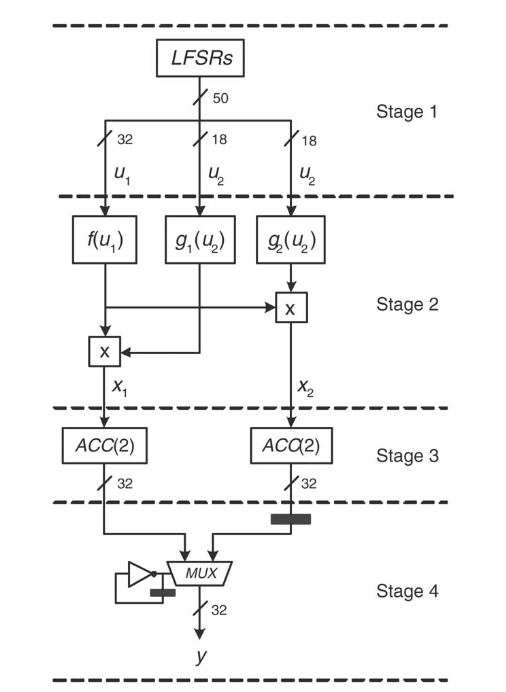
\includegraphics[height=20em]
{Figures/noise_gen_architecture.png}
\caption[Hardware architecture of an AWGN generator]
{Hardware architecture of an AWGN generator. Image taken from \cite{noise_gen}}
\label{Figure:NoiseGeneration:NoiseGenArchitecture}
\end{figure}
%%%%%%%%%%%%%%%%%%%%%%%%%%%%%%%%%%%%%%%%%%%%%%%%%%%%%%%%%%%%%%%%% 

The overall hardware architecture can be divided into four stages (see \Figure~\fref{Figure:NoiseGeneration:NoiseGenArchitecture}). Henceforth we discuss an implementation using 32 bits for precision. The only inputs driving this design are a clock, and the output is a 32 bit fixed point (4 integer bits and 28 fraction bits) representation of a normally distributed sample. 

\subsection{Stage I}

This stage generates the uniform random variables that get transformed using the approximated Box Muller method. This is implemented using Tausworthe generators \cite{noise_gen} which implement high periodicity uniform random samples using linear shift registers. These generators will output two 32 bit sequences that are interpreted as a fixed point float (all 32 bits fraction).

\subsection{Stage II}
In this stage, the Box Muller transform is applied to the two input RVs. The functions involved are segmented and approximated linearly. The output of these functions are then multiplied, generating two normally distributed samples.

%%%%%%%%%%%%%%%%%%%%%%%%%%%%%%%%%%%%%%%%%%%%%%%%%%%%%%%%%%%%%%%%%
% FIGURE: Noise Generation: F segmentation
\begin{figure}
\centering\CaptionFontSize
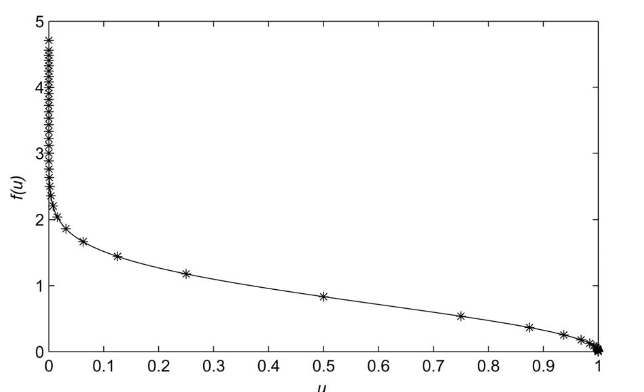
\includegraphics[height=15em]
{Figures/f_segmentation.png}
\caption[Non-uniform segmentation of f(u)]
{Non-uniform segmentation of f(u). Image taken from \cite{noise_gen}}
\label{Figure:NoiseGeneration:FSegmentation}
\end{figure}
%%%%%%%%%%%%%%%%%%%%%%%%%%%%%%%%%%%%%%%%%%%%%%%%%%%%%%%%%%%%%%%%% 
\TODO{cite}

The function f is segmented by placing segment boundaries at $0$, $2^{-n}$ for  $0 < n < 32$, $1-2^{-n}$ for $1<n<32$, and $1$ resulting in the domain being split into 62 segments. (\Figure~\fref{Figure:NoiseGeneration:FSegmentation})) is a graphical representation of this segmentation. Linear coefficients of these segments are stored in read only memory (ROM) addressed 0 to 61. To efficiently calculate an input’s segment and corresponding address in the ROM we employ a chain of OR and AND gates on the bits of the input as shown in an 8 bit example in \Figure~\fref{Figure:NoiseGeneration:AddressCalculator}). Each entry of the ROM has four values of interest: two base values and two scaling values for the first and zero-th order coefficients. Putting it all together, given an input $u$, $f(u)$ is evaluated by 

%%%%%%%%%%%%%%%%%%%%%%%%%%%%%%%%%%%%%%%%%%%%%%%%%%%%%%%%%%%%%%%%%
% FIGURE: Noise Generation: Address Calculator
\begin{figure}
\centering\CaptionFontSize
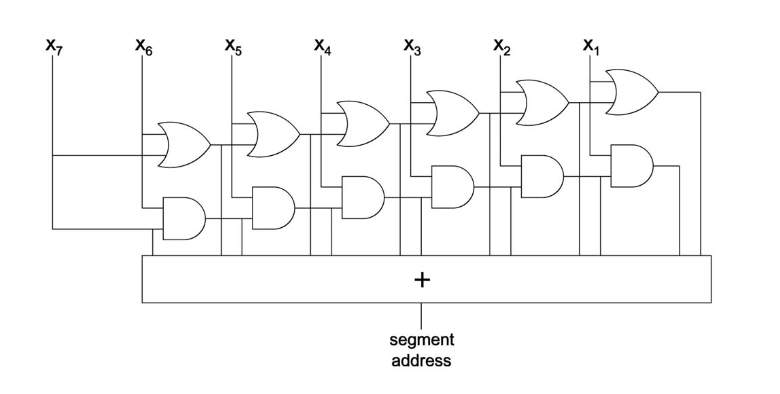
\includegraphics[height=15em]
{Figures/address_calculator.png}
\caption[8-bit example segment address calculator for non-uniform segmentation]
{8-bit example segment address calculator for non-uniform segmentation. Image taken from \cite{noise_gen}}
\label{Figure:NoiseGeneration:AddressCalculator}
\end{figure}
%%%%%%%%%%%%%%%%%%%%%%%%%%%%%%%%%%%%%%%%%%%%%%%%%%%%%%%%%%%%%%%%% 
\TODO{cite}

\begin{enumerate}
    \item Passing $u$ through the segment address calculator
    \item Reading the ROM at the address to obtain the linear coefficients of the corresponding segment: $c_{s1}$, $c_1$, $c_{s0}$, $c_0$ (calculated and flashed onto the board).
    \item Outputting the linear approximation $f(u) = 2^{(c_{s1})} (c_1 * u) + 2^{(c_{s0})} (c_0 )$
\end{enumerate}

%%%%%%%%%%%%%%%%%%%%%%%%%%%%%%%%%%%%%%%%%%%%%%%%%%%%%%%%%%%%%%%%%
% FIGURE: Noise Generation: G Symmetry
\begin{figure}
\centering\CaptionFontSize
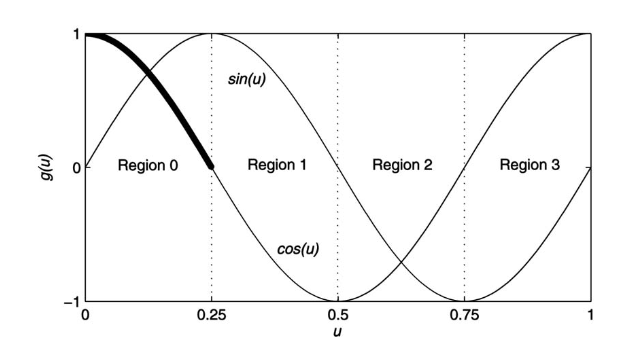
\includegraphics[height=15em]
{Figures/g_symm.png}
\caption[Illustration of the symmetry of $g_1$ and $g_2$]
{Illustration of the symmetry of $g_1$ and $g_2$. Image taken from \cite{noise_gen}}
\label{Figure:NoiseGeneration:GSymmetry}
\end{figure}
%%%%%%%%%%%%%%%%%%%%%%%%%%%%%%%%%%%%%%%%%%%%%%%%%%%%%%%%%%%%%%%%% 
\TODO{cite}

Due to symmetry of sin and cosine (\Figure~\fref{Figure:NoiseGeneration:GSymmetry})), functions $g_1$ and $g_2$ can both be evaluated just by performing approximations on the first $\frac{1}{4}$ of the domain of $g_2$. Below is a graphical representation of how this domain is segmented. Here we first uniformly segment the domain into 4 intervals and within each interval employ the same segmentation architecture described for $f$. For the first three intervals we segment into 6, and for the last segment we only segment into three (in architecture this corresponds to disconnecting certain branches from the adder). Aside from segmenting, everything pertaining to function evaluation is identical to $f$ except that the appropriate symmetry transformations are done to the linear approximation in order to obtain $g_1(u)$ and $g_2(u)$. We also drop the $\sqrt{2}$ multiplier in front of both functions due to the implementation of stage 3.

%%%%%%%%%%%%%%%%%%%%%%%%%%%%%%%%%%%%%%%%%%%%%%%%%%%%%%%%%%%%%%%%%
% FIGURE: Noise Generation: G Segmentation
\begin{figure}
\centering\CaptionFontSize
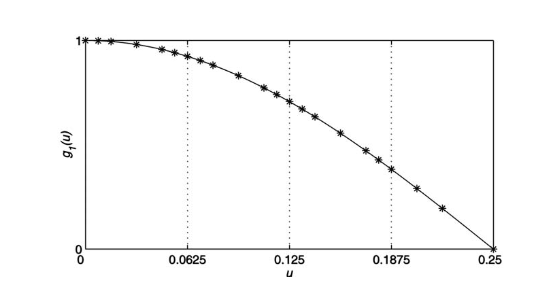
\includegraphics[height=15em]
{Figures/g_segmentation.png}
\caption[Non-uniform segmentation of Region 0 of $g$]
{Non-uniform segmentation of Region 0 of $g$. Image taken from \cite{noise_gen}}
\label{Figure:NoiseGeneration:GSegmentation}
\end{figure}
%%%%%%%%%%%%%%%%%%%%%%%%%%%%%%%%%%%%%%%%%%%%%%%%%%%%%%%%%%%%%%%%% 
\TODO{cite}

After having obtained approximated evaluations of $f(u_1)$, $g_1(u_2)$, and $g_2(u_2)$ we simply multiply the values together to obtain $x_1$ and $x_2$.

\subsection{Stage III}
In this stage we implement a small-scale application of the central limit theorem (CLT) and add successive outputs of the previous stage together. This is done in hardware using a size 2 accumulator for the $x_1$ outputs and another one for the x2 outputs. These will output the sum of the last two $x_1$ and $x_2$ samples generated which allows us to slightly employ CLT to introduce more normality in the samples while at the same time getting rid of need for the 
$\sqrt{2}$ multiplication in $g_1$ and $g_2$. Note that the output of this stage now generates two valid AWGN samples every other cycle; we fix this in stage 4.
\subsection{Stage IV}
This stage functions to alternate the outputs of stage 3 such that a sample is generated every cycle. This is done by simply buffering one output and then using a multiplexor to switch between the buffered output and the non-buffered output every cycle.

\section{Results and Future Work}

Running simulations of performance using this architecture, we see that it produces highly accurate AWGN samples. In our implementation, the approximations of the functions $f$, $g_1$, and $g_2$ have worst case absolute errors of 0.016, 0.0012, and 0.0012 respectively (see \Figure~\fref{Figure:NoiseGeneration:ApproximationError}). 

%%%%%%%%%%%%%%%%%%%%%%%%%%%%%%%%%%%%%%%%%%%%%%%%%%%%%%%%%%%%%%%%%
% FIGURE: Noise Generation: Approximation Error
\begin{figure}
\centering\CaptionFontSize
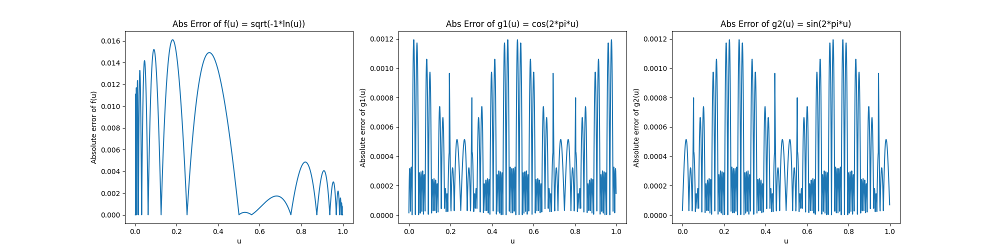
\includegraphics[width=\textwidth]
{Figures/approx_error.png}
\caption[Absolute error between hardware approximations and true value of $f$, $g_1$, and $g_2$]
{Absolute error between hardware approximations and true value of $f$, $g_1$, and $g_2$}
\label{Figure:NoiseGeneration:ApproximationError}
\end{figure}
%%%%%%%%%%%%%%%%%%%%%%%%%%%%%%%%%%%%%%%%%%%%%%%%%%%%%%%%%%%%%%%%% 

Furthermore, we are able to perform the Box-Muller method with high accuracy. \Figure~\fref{Figure:NoiseGeneration:UniformSamples} shows samples of a uniform distribution generated by the Tausworthe generators in stage 1 that get transformed into normally distributed samples at the output of stage 4 (\Figure~\fref{Figure:NoiseGeneration:NormalSamples}). These samples fit a normal distribution very well having only a 0.03 deviation from unit variance.

%%%%%%%%%%%%%%%%%%%%%%%%%%%%%%%%%%%%%%%%%%%%%%%%%%%%%%%%%%%%%%%%%
% FIGURE: Noise Generation: Uniform Samples
\begin{figure}
\centering\CaptionFontSize
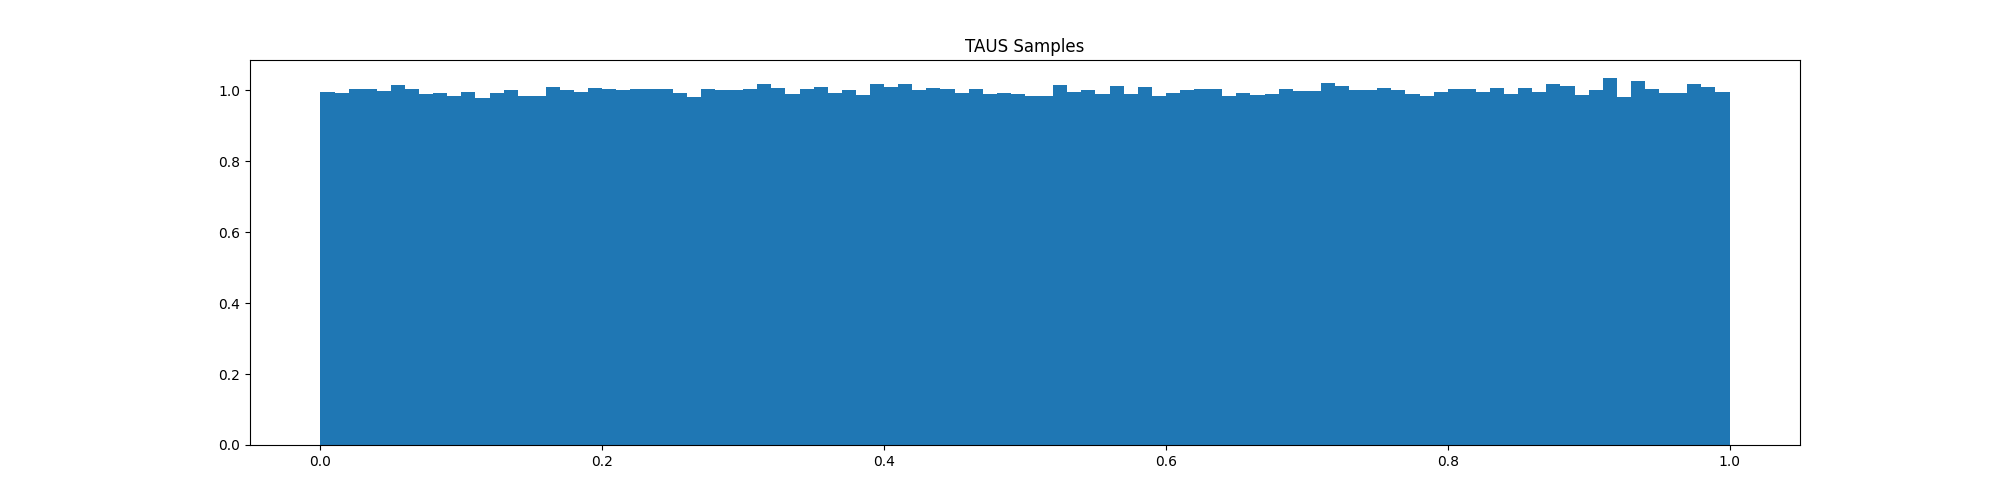
\includegraphics[width=\textwidth]
{Figures/uniform_dist.png}
\caption[Uniform random samples generated in hardware using a Tausworthe generator]
{Uniform random samples generated in hardware using a Tausworthe generator.}
\label{Figure:NoiseGeneration:UniformSamples}
\end{figure}
%%%%%%%%%%%%%%%%%%%%%%%%%%%%%%%%%%%%%%%%%%%%%%%%%%%%%%%%%%%%%%%%% 
%%%%%%%%%%%%%%%%%%%%%%%%%%%%%%%%%%%%%%%%%%%%%%%%%%%%%%%%%%%%%%%%%
% FIGURE: Noise Generation: Normal Samples
\begin{figure}
\centering\CaptionFontSize
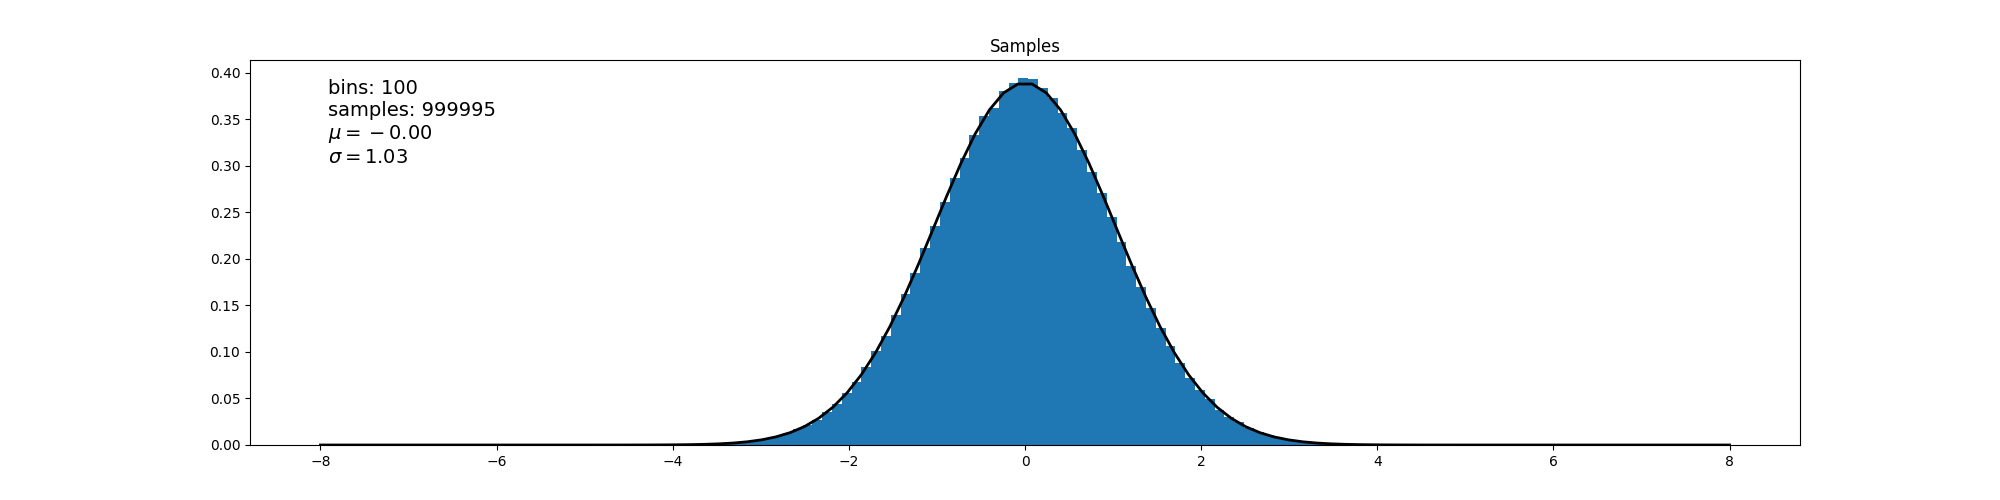
\includegraphics[width=\textwidth]
{Figures/normal_dist.png}
\caption[Normal random samples generated in hardware Box-Muller method implementation]
{Normal random samples generated in hardware Box-Muller method implementation}
\label{Figure:NoiseGeneration:NormalSamples}
\end{figure}
%%%%%%%%%%%%%%%%%%%%%%%%%%%%%%%%%%%%%%%%%%%%%%%%%%%%%%%%%%%%%%%%% 

Going forward we would like to examine the performance of this architecture at the tails of the distribution, an area that is quintessentially difficult to reproduce very well. Furthermore, there is room for improvement in terms of accuracy of the function evaluators. \cite{noise_gen} is able to reduce the absolute errors shown here by half and utilize less space on hardware, an effort that with more time can be accomplished with slight changes to the coefficient storage and calculation.
